\documentclass[10pt]{article}
%%%%%%%%%%%%%%%%%%%%%%%%%%%%%%%%%%%%%%%%
\usepackage{amsmath}
\usepackage{verbatim}
\usepackage[usenames,dvipsnames]{color}
\usepackage{ulem}
\usepackage{setspace}
\usepackage{lscape}
\usepackage{longtable}
\usepackage[top=1.25in,bottom=1.5in,left=1in,right=1.5in,landscape]{geometry}
\usepackage{graphicx}
\usepackage{epstopdf}
\usepackage[usenames,dvipsnames]{pstricks}
\usepackage{epsfig}
\usepackage{pstricks-add}
\usepackage{pst-node}
\usepackage{fancyhdr}
\usepackage[absolute,showboxes]{textpos}

%TCIDATA{OutputFilter=LATEX.DLL}
%TCIDATA{Version=5.00.0.2552}
%TCIDATA{<META NAME="SaveForMode" CONTENT="1">}
%TCIDATA{Created=Thursday, August 28, 2003 13:38:44}
%TCIDATA{LastRevised=Thursday, August 14, 2008 15:20:27}
%TCIDATA{<META NAME="GraphicsSave" CONTENT="32">}
%TCIDATA{<META NAME="DocumentShell" CONTENT="Standard LaTeX\Blank - Standard LaTeX Article">}
%TCIDATA{Language=American English}
%TCIDATA{CSTFile=LaTeX article (bright).cst}

\setcounter{MaxMatrixCols}{10}

\newenvironment{proof}[1][Proof]{\noindent\textbf{#1.} }{\ \rule{0.5em}{0.5em}}
\setlength{\columnsep}{.2in}

\renewcommand{\labelitemii}{$\cdot$}

\pagestyle{fancy} \fancyhead{} \fancyfoot{} \rfoot{} \lfoot{}

\newcommand{\slide}[2]{
\begin{textblock}{11}(0,0)
\textcolor{Black}{\textbf{\huge \rule{0pt}{1in} \raisebox{.2in}{#1}}}
\end{textblock}
\begin{Large} \noindent
#2
\end{Large}
\vfill \pagebreak}

\setlength{\TPHorizModule}{1in}
\setlength{\TPVertModule}{1in}
\textblockcolour{Yellow}
\renewcommand{\headrulewidth}{0pt}



\begin{document}
\onehalfspacing 

\lfoot{Technological Growth} \rfoot{Economic Growth}

\slide{Technology Drives Growth}{In the Solow model, the only thing that produces trend growth is technology, $A$. We said that $A$ grew at some rate $g$ over time. Where does $g$ come from?

\vspace{.25in}\noindent Think of $A$ as ideas of how to combine inputs more efficiently. Better ideas, higher output per worker. So we need to continue to have new ideas to grow.

\vspace{.25in}\noindent Economics of ideas are different from economics of goods and services
\begin{itemize}
	\item Ideas are non-rival. I can use the idea of calculus at the same time as you. 
	\item Ideas are (generally) non-exclusive. I cannot stop you from using calculus.
\end{itemize}

\vspace{.25in}\noindent Because ideas are so different, the economics of producing ideas are different from our standard world of perfect competition. 
}

\slide{Economics of Ideas}{Idea are non-rival. Produce them once, and then anyone can use them.
\begin{itemize}
	\item Ideas have high fixed costs. It took a lot of effort to invent calculus or a new drug. 
	\item Ideas have low (zero) marginal costs. It cost nothing for you to use calculus now. It costs very little to produce one more pill.
\end{itemize}

\vspace{.25in}\noindent The combination of fixed costs and low marginal costs mean ideas have \textit{increasing returns to scale}.

\vspace{.25in}\noindent Increasing returns to scale implies that the average cost of the idea (or good that embodies the idea) is higher than the marginal cost of reproducing the idea (or good that embodies the idea)

\vspace{.25in}\noindent So ideas (or the goods embodying them) will only be produced if someone can charge more than marginal cost. In other words, there must be \textit{imperfect competition}.
}

\slide{Imperfect Competition}{Firms that produce ideas, or goods that embody ideas (like pills, or Microsoft Office, or an iPhone) earn profits by charging a price for the good over marginal cost.

\vspace{.25in}\noindent The profits are there to make up for the large fixed cost to coming up with the idea.

\vspace{.25in}\noindent Can only sustain these profits by preventing others from using the idea -- patents, branding, marketing, copyrights, etc.. 

\vspace{.25in}\noindent Without protection for the idea, firms will not earn profits. Without profits, firms will not undertake fixed cost of R\&D to invent new product. 

\vspace{.25in}\noindent So the growth of ideas, $A$, depends on there being imperfect competition. Economic growth fundamentally relies on market imperfections.
}

\slide{Population and Ideas}{Population is a positive for ideas
\begin{itemize}
	\item More people means more researchers, thinkers, inventors, etc..
	\item Ideas are non-rival. So more people does not mean fewer ideas for each of us. We can all use all the ideas all the time. Note difference from capital.
	\item More people means larger markets. Larger markets mean more profits for firms that use ideas. More profits means more investment in R\&D.
\end{itemize} 

\vspace{.25in}\noindent All together, population (or scale) will be a \textit{positive} contributor to growth. 
}

\slide{Data on Ideas?}{Number of patents issued in the U.S.
\begin{center}
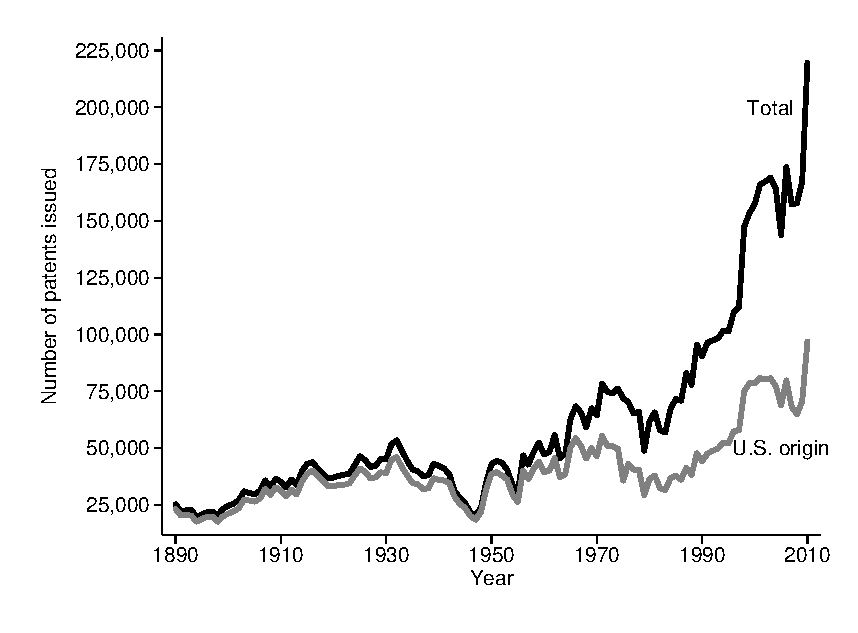
\includegraphics[scale=1.2]{figure_4_5.eps}
\end{center}
}

\slide{Data on Ideas?}{Number of scientists and engineers doing R\&D in U.S. and G-5.
\begin{center}
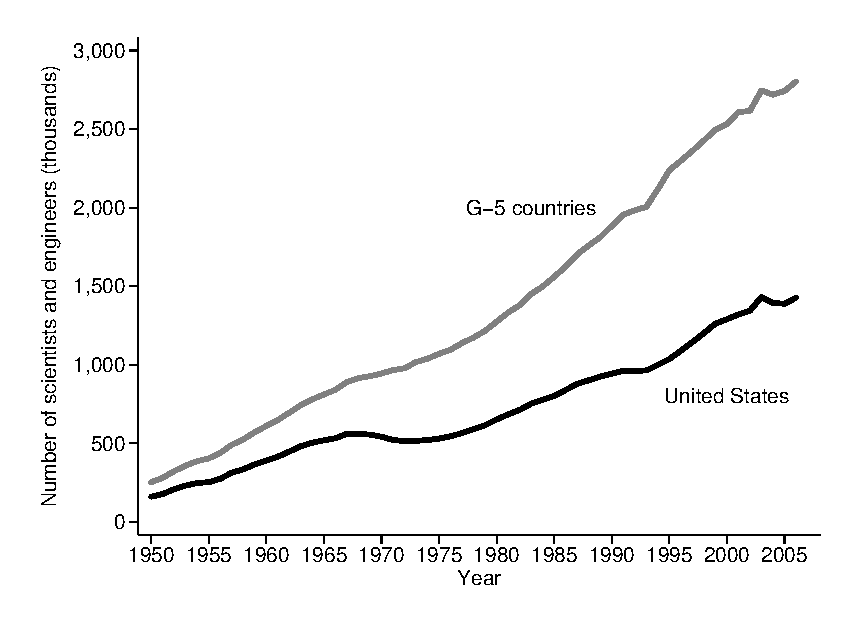
\includegraphics[scale=1.2]{figure_4_6.eps}
\end{center}
}

\slide{Ideas and Trend Growth}{Note that while the number of ideas, and number of researchers is climbing very rapidly, trend growth in the U.S. has remained very steady. Will want to ensure our model captures that.
\begin{center}
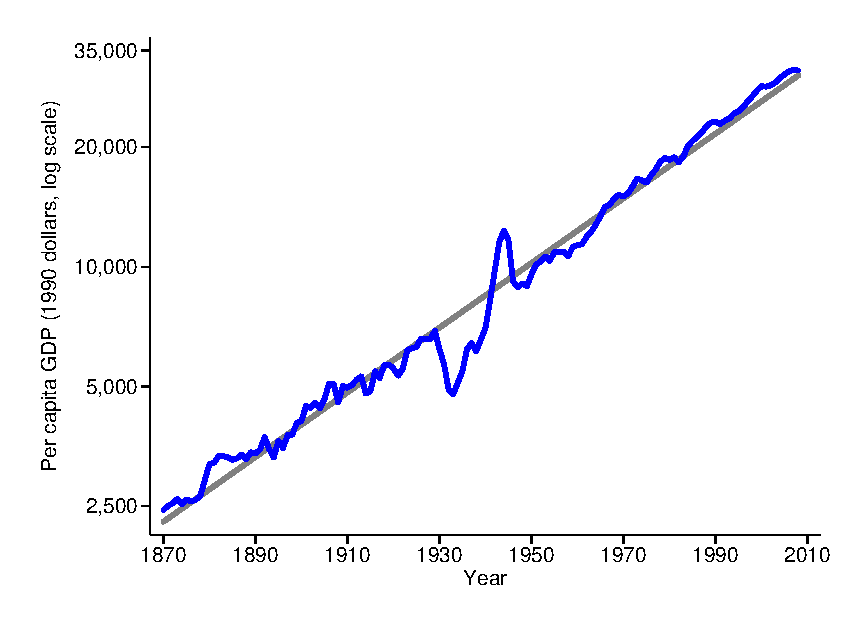
\includegraphics[scale=1.2]{figure_1_4.eps}
\end{center}
}

\slide{Modelling Ideas}{We want some model of the accumulation of ideas. $A$ is the index of ``ideas''. How do we accumulate new ideas? Model will have two parts:
\begin{itemize}
	\item Mechanics of accumulating technology - which will depend on R\&D effort exerted
	\item Economics of how much effort to exert on R\&D
\end{itemize}

\vspace{.25in}\noindent Start with mechanics - and this will be sufficient to determine the long-run growth rate $g$ in the economy.
}

\slide{Accumulation of $A$}{If $A$ is the stock of technoloy (ideas) at any given time, then we'll assume that
\begin{equation}
\dot{A} = \overline{\theta} L_A
\end{equation}
where $L_A$ are the number of workers (researchers) doing R\&D on new technologies, and $\overline{\theta}$ is the rate at which each researcher finds a new idea.

\vspace{.25in}\noindent $\overline{\theta}$ depends on 
\begin{itemize}
	\item Total number of researchers working (perhaps duplicating efforts, or economies of scale)
	\item The existing level of technology, $A$
\end{itemize}
}

\slide{Determinants of $\overline{\theta}$}{We'll let 
\begin{equation}
\overline{\theta} = \theta L_A^{\lambda-1} A^{\phi}
\end{equation}
so that
\begin{equation}
\dot{A} = \theta L_A^{\lambda} A^{\phi}
\end{equation}
or the growth rate of $A$ is
\begin{equation}
\frac{\dot{A}}{A} = \theta \frac{L_A^\lambda}{A^{1-\phi}}
\end{equation}
}

\slide{Interpretations}{Change in $A$ is
\begin{equation}
\dot{A} = \theta L_A^{\lambda} A^{\phi}.
\end{equation}
\begin{itemize}
	\item $0<\lambda<1$: This captures how much research responds to number of researchers. If $\lambda=0$, adding researchers doesn't change rate at which technology grows. If $\lambda>0$ then adding researchers raises technological growth, but $\lambda<1$ implies some congestion/duplication.
	\item $\phi<1$. $\phi$ captures effect of technology level on change in technology
	\begin{itemize}
		\item $\phi>0$: ``standing on shoulders'' 
		\item $\phi<0$: ``fishing out''
		\item $\phi=0$: effects offset each other
	\end{itemize}
\end{itemize}
}

\slide{Long-run Growth Rate}{What is the growth rate of $A$ along a balanced growth path? Meaning, what is the growth rate of $A$ such that $\dot{A}/A$ remains constant? 
\begin{equation}
\frac{\dot{A}}{A} = \theta \frac{L_A^\lambda}{A^{1-\phi}}
\end{equation}
$\dot{A}/A$ will be constant if $L_A^\lambda$ grows at exactly the same rate as $A^{1-\phi}$. Take logs and derivatives of both sides
\begin{eqnarray}
\ln (\dot{A}/A) &=& \ln{\theta} + \lambda \ln{L_A} - (1-\phi)\ln{A} \\
\frac{\partial \ln (\dot{A}/A)}{\partial t} = \lambda \frac{\dot{L_A}}{L_A} - (1-\phi)\frac{\dot{A}}{A}.
\end{eqnarray}

\vspace{.25in}\noindent Along the BGP, we want the growth rate of $A$ to be constant, or the left-hand side should be zero. This means that along the BGP we want
\begin{equation}
\lambda \frac{\dot{L_A}}{L_A} - (1-\phi)\frac{\dot{A}}{A} = 0
\end{equation}
which we can solve for
\begin{equation}
\frac{\dot{A}}{A} = \frac{\lambda}{1-\phi}\frac{\dot{L_A}}{L_A}.
\end{equation}
}

\slide{Long-Run Growth Rate}{Given
\begin{equation}
\frac{\dot{A}}{A} = \frac{\lambda}{1-\phi}\frac{\dot{L_A}}{L_A}.
\end{equation}
we see that the growth rate of $A$ along the BGP depends on the growth rate of researchers. What is the growth rate of $L_A$? It can only be
\begin{equation}
\frac{\dot{L_A}}{L_A} = n
\end{equation}
along the BGP. If $\dot{L_A}/L_A>n$, then eventually 100\% of workers would be researchers, and no one would do any production work. This implies that
\begin{equation}
\frac{\dot{A}}{A} = \frac{\lambda}{1-\phi}n
\end{equation}
is the long-run trend growth rate.
}

\slide{Trend Growth}{Given
\begin{equation}
\frac{\dot{A}}{A} = \frac{\lambda}{1-\phi}n
\end{equation}
note that trend growth is a positive function of $n$. That is, the faster population grows, the faster technology grows. Why? Because more people means more researchers, and more researchers means more ideas. 

\vspace{.25in}\noindent To see a little more intution, set $\lambda = 1$ and $\phi = 0$. So we have
\begin{equation}
\dot{A} = \theta L_A
\end{equation}
and
\begin{equation}
\frac{\dot{A}}{A} = n
\end{equation}

\vspace{.25in}\noindent Top equation says that the absolute change in technology is proportional to the number of researchers. Without $L_A$ rising, eventually $\dot{A}/A$ would equal zero. Only with population growth, and growth in $L_A$, will technolgy continue to grow.

}

\slide{Special Case}{Romer's original growth model set $\lambda=1$ and $\phi=1$, for
\begin{equation}
\dot{A} = \theta L_A A
\end{equation}
or
\begin{equation}
\frac{\dot{A}}{A} = \theta L_A.
\end{equation}
For Romer, an increase in the number of researchers led to an increase in the \textit{growth rate} of technology. If this were true, then the trend growth rate of output per worker should have been rising over the 20th century.

\vspace{.25in}\noindent Because growth rate is so steady over modern history, the assumption that $\phi=1$ cannot be right. Almost certain that $\phi<1$.
}

\slide{A Little Economics}{So far, this description is completely mechanical. $g$ depends on the values of $\lambda$, $\phi$, and $n$. Aren't there economic choices to be made?

\vspace{.25in}\noindent Yes. The choice we'll focus on is what fraction of the total labor force is actually used to do research. Let
\begin{equation}
L_A = s_R L
\end{equation}
where $s_R$ is like a savings rate. $0<s_R<1$ is the fraction of workers doing R\&D.

\vspace{.25in}\noindent If $\phi<1$, then $s_R$ has no effect on the long-run \textit{growth rate} of $A$, only on the \textit{level} of $A$.
}

\slide{Analyzing the Change}{We assume that $\lambda = 1$ and $\phi=0$, so
\begin{equation}
\frac{\dot{A}}{A} = \frac{\theta s_R L}{A}.
\end{equation}
\vspace{.25in}\noindent What happens if $s_R$ goes up to $s_R'$?
\begin{center}
\scalebox{1}{
\begin{pspicture}(10,10)
\psline{->}(0,0)(10,0) \psline{->}(0,0)(0,10)
\psline(0,4)(10,4) \psline(0,0)(8,8)
\psline[linestyle=dotted](6.67,0)(6.67,6.67) \psline[linestyle=dotted](4,0)(4,4)
\rput(-.6,4){$g = n$} \rput(0,10.3){$\dot{A}/A$} \rput(10.5,0){$L_A/A$}
\rput(8,8.3){$\dot{A}/A = \theta L_A/A$} \rput(4,-.3){$g/\theta$} \rput(6.67,-.3){$s_R'L_0/A_0$}
\psline[arrowscale=2]{<-}(4.2,4.2)(5,5) \psline[arrowscale=2]{<-}(4.8,4.8)(5.4,5.4) \psline[arrowscale=2]{<-}(5.4,5.4)(6,6) \psline[arrowscale=2]{<-}(6,6)(6.4,6.4)
\psline[arrowscale=2,linestyle=dashed,dash=3pt 2pt]{->}(4.3,1)(6.5,1)
\end{pspicture}
}
\end{center}
}

\slide{Temporary Growth effect}{The shift up in $s_R$ has a temporary effect on the \textit{growth rate} of $A$, but does not change the long-run growth rate. Eventually it must be that $g = \dot{A}/A = n$ again.

\vspace{.25in}\noindent
\begin{center}
\scalebox{1}{
\begin{pspicture}(10,10)
\psline{->}(0,0)(10,0) \psline{->}(0,0)(0,10)
\psline(0,4)(3,4) \pscurve(3,6)(4,5)(10,4) \psline[linestyle=dotted](3,6)(3,0)
\rput(3,-.3){$t=0$} \rput(0,10.3){$\dot{A}/A$} \rput(10.5,0){Time} 
\rput(-.3,4){$n$}
\end{pspicture}
}
\end{center}
}

\slide{Level Effect}{The shift up in $s_R$ does permanently raise the \textit{level} of $A$.

\vspace{.25in}\noindent
\begin{center}
\scalebox{1}{
\begin{pspicture}(10,10)
\psline{->}(0,0)(10,0) \psline{->}(0,0)(0,10) 
\psline(1,.25)(2.5,1) \psline[linestyle=dashed,dash=3pt 2pt](2.5,1)(9.5,4.5)
\pscurve(2.5,1)(3,2)(4,3)(8,5)(10,6)
\rput(0,10.3){Log $A$} \rput(10.5,0){Time}
\psbrace[nodesepA=5pt](9.5,4.5)(9.5,5.75){Level effect}
\end{pspicture}
}	
\end{center}
}

\slide{Embedding in Solow Model}{We now have model for technology growth. How does that fit in the Solow model? One change to make. With $s_R$ people researching, only $(1-s_R)$ are working, so 
\begin{equation}
y = k^{\alpha}(A(1-s_R)L)^{1-\alpha}
\end{equation}
and along the balanced growth path
\begin{equation}
y(t) = A(t) (1-s_R)\left(\frac{s}{\delta +n +g} \right)^{\alpha/(1-\alpha)},
\end{equation}
Fewer people working means lower output per worker. 
}

\slide{Incorporating Endogenous Technology}{Repeating
\begin{equation}
y(t) = A(t) (1-s_R)\left(\frac{s}{\delta +n +g} \right)^{\alpha/(1-\alpha)},
\end{equation}

\vspace{.25in}\noindent What is $A(t)$? Along the BGP we know that $\dot{A}/A = g$. This means that
\begin{equation}
g = \frac{s_R L}{A}
\end{equation}
along the BGP. We can rearrange to find the value of $A$ along that balanced growth path
\begin{equation}
	A(t) = \frac{s_R L(t)}{g}
\end{equation}
where we added $(t)$ to be clear that $A$ is growing along with population over time.

\vspace{.25in}\noindent Add to the BGP for $y(t)$ above to get
\begin{equation}
y(t) = \frac{s_R L(t)}{g} (1-s_R) \left(\frac{s}{\delta +n +g} \right)^{\alpha/(1-\alpha)}
\end{equation}
}

\slide{Implications}{Repeat
\begin{equation}
y(t) = \frac{s_R L(t)}{g} (1-s_R) \left(\frac{s}{\delta +n +g} \right)^{\alpha/(1-\alpha)}
\end{equation}
and what do we see?
\begin{itemize}
	\item $s_R$ has conflicting effects on the level of output per capita. You can do so much research that the leve of $y(t)$ actually goes down because of a lack of workers.
	\item Conflicting effects of population. There are scale effects, so if $L(t)$ is bigger, we have higher output \textit{per worker}. More people means more ideas.
	\item Faster population \textit{growth} means a lower \textit{level} of output per worker. Recall that $g = n$. Fast-growing populations increase $A$ so fast that it makes it harder to find new technologies. Also dilutes capital per worker as in Solow.
\end{itemize}
}

\end{document}